\chapter{Multipath Propagation \& Fading (Rayleigh \& Rician)}
\label{ch:multipath-propagation-fading}

\begin{nontechnical}
\textbf{Multipath is like hearing echoes in a canyon}---radio signals bounce off buildings and walls, arriving at your phone from multiple directions at slightly different times.

\textbf{The problem:}
\begin{enumerate}
\item Signal travels \textbf{direct path} from tower to phone (fast)
\item Same signal bounces off buildings (slower paths)
\item All copies arrive at different times and \textbf{interfere}
\item Sometimes they add up (strong signal), sometimes they cancel out (weak signal)
\item This causes \textbf{fading}: signal strength fluctuates wildly as you move
\end{enumerate}

\textbf{Real-world experience:}
\begin{itemize}
\item \textbf{Driving through city:} Cell signal goes from 5 bars to 2 bars back to 5 bars---that's multipath fading
\item \textbf{WiFi dead spots:} Walk 1 meter and signal drops---destructive interference from multipath
\item \textbf{Crackling old TV:} Picture would fade in/out---multipath from distant transmitter
\end{itemize}

\textbf{Two types:}
\begin{itemize}
\item \textbf{Rayleigh fading} (no direct path): All paths bounced/scattered, signal varies randomly (can drop 30+ dB), common in dense urban areas
\item \textbf{Rician fading} (strong direct path + echoes): One dominant line-of-sight path plus weaker echoes, less severe fading, common in open areas
\end{itemize}

\textbf{How engineers fix it:} MIMO (multiple antennas), OFDM (spread data across frequencies), adaptive coding, and interleaving.
\end{nontechnical}

\section{Overview}

\textbf{Multipath propagation} occurs when RF signals reach the receiver via \textbf{multiple paths} simultaneously, each with different:
\begin{itemize}
\item \textbf{Delay} (arrival time)
\item \textbf{Amplitude} (path loss)
\item \textbf{Phase} (due to different path lengths)
\end{itemize}

\begin{keyconcept}
Signals combine \textbf{constructively} or \textbf{destructively}, causing \textbf{fading}---rapid signal strength variations that can degrade bit error rate by 1000$\times$ compared to AWGN channels. This is the dominant impairment in mobile and urban wireless communications.
\end{keyconcept}

\textbf{Critical applications:} Cellular networks, WiFi, mobile satellite, and any NLOS (non-line-of-sight) communication system.

\subsection{Multipath Propagation Visualization}

\begin{center}
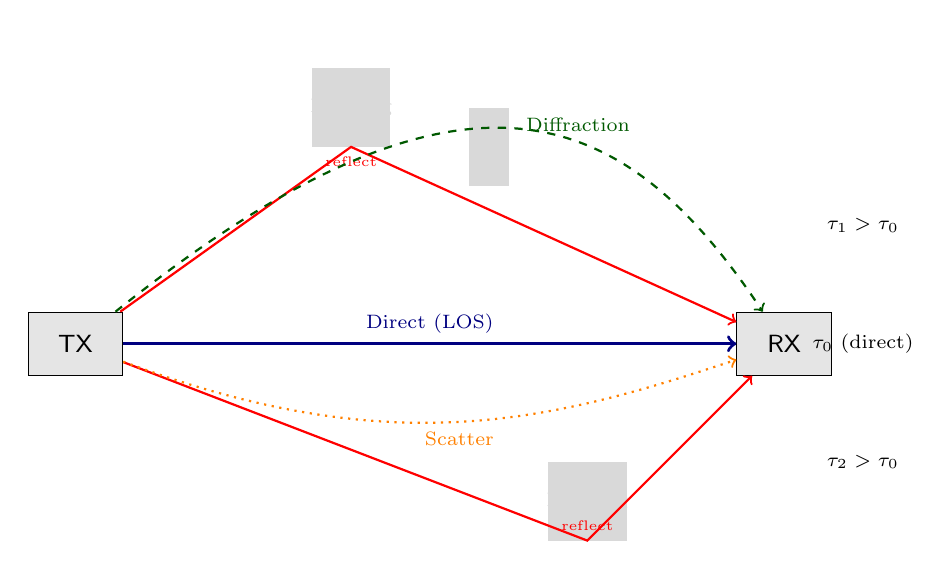
\begin{tikzpicture}[scale=1.0,
  node distance=1.5cm,
  block/.style={rectangle, draw, minimum width=1.2cm, minimum height=0.8cm, font=\sffamily\small},
  path/.style={->, thick}
]

% Transmitter
\node[block, fill=black!10] (tx) at (0,0) {TX};

% Receiver
\node[block, fill=black!10] (rx) at (9,0) {RX};

% Buildings/obstacles
\fill[gray!30] (3,2.5) rectangle (4,3.5) node[midway,font=\scriptsize] {Building};
\fill[gray!30] (6,-2.5) rectangle (7,-1.5) node[midway,font=\scriptsize] {Building};
\fill[gray!30] (5,2) rectangle (5.5,3) node[midway,font=\scriptsize,rotate=90] {Wall};

% Direct path (LOS)
\draw[path, NavyBlue, very thick] (tx) -- node[above,font=\scriptsize,pos=0.5] {Direct (LOS)} (rx);

% Reflected paths
\draw[path, Red] (tx) -- (3.5,2.5) node[pos=1,below,font=\tiny] {reflect} -- (rx);
\draw[path, Red] (tx) -- (6.5,-2.5) node[pos=1,above,font=\tiny] {reflect} -- (rx);

% Diffracted path
\draw[path, Green!70!black, dashed] (tx) .. controls (5,4) and (7,3) .. node[above,font=\scriptsize,pos=0.6] {Diffraction} (rx);

% Scattered path
\draw[path, orange, dotted] (tx) .. controls (4,-1.5) and (6,-1) .. node[below,font=\scriptsize,pos=0.5] {Scatter} (rx);

% Time annotations
\node[font=\scriptsize,align=left] at (10,0) {$\tau_0$ (direct)};
\node[font=\scriptsize,align=left] at (10,1.5) {$\tau_1 > \tau_0$};
\node[font=\scriptsize,align=left] at (10,-1.5) {$\tau_2 > \tau_0$};

\end{tikzpicture}
\end{center}

\section{Physical Mechanisms}

\subsection{Reflection}

\textbf{EM waves bounce off surfaces:}
\begin{itemize}
\item \textbf{Ground} (two-ray model)
\item \textbf{Buildings} (urban canyons)
\item \textbf{Water} (maritime communications)
\item \textbf{Ionosphere} (HF skywave)
\end{itemize}

\textbf{Reflection coefficient} depends on:
\begin{itemize}
\item Polarization (horizontal vs vertical)
\item Angle of incidence
\item Surface material (conductivity, permittivity)
\end{itemize}

\begin{calloutbox}{Example: Concrete Wall Reflection}
Concrete wall at 2.4~GHz: reflection coefficient $\approx 0.3$--$0.5$ (corresponding to 3--6~dB loss per bounce).
\end{calloutbox}

\subsection{Diffraction}

\textbf{Bending around obstacles} (Fresnel diffraction):
\begin{itemize}
\item Building edges
\item Hills/terrain
\item Trees
\end{itemize}

\textbf{Knife-edge diffraction loss:}
\begin{equation}
L_d \approx 6 + 20\log_{10}\left(\sqrt{(v-0.1)^2 + 1} + v - 0.1\right) \quad \text{(dB)}
\label{eq:knife-edge-diffraction}
\end{equation}
where:
\begin{itemize}
\item $v$ = Fresnel-Kirchhoff diffraction parameter (dimensionless)
\item $L_d$ = diffraction loss (dB)
\end{itemize}

\textbf{Implication:} Signals can ``bend'' into shadowed regions, enabling NLOS coverage.

\subsection{Scattering}

\textbf{Interaction with rough surfaces or small objects:}
\begin{itemize}
\item Rough terrain (vegetation, rocks)
\item Lamp posts, signs
\item Rain/fog droplets (at high frequencies)
\end{itemize}

\textbf{Rayleigh scattering} (object size $\ll \lambda$):
\begin{equation}
P_{\text{scattered}} \propto \frac{1}{\lambda^4}
\label{eq:rayleigh-scattering}
\end{equation}
where:
\begin{itemize}
\item $P_{\text{scattered}}$ = scattered power
\item $\lambda$ = wavelength
\end{itemize}

\begin{calloutbox}{Example: Blue Sky}
The blue color of the sky results from Rayleigh scattering of visible light by air molecules---shorter wavelengths (blue) scatter more than longer wavelengths (red).
\end{calloutbox}

\section{Time-Domain Effects}

\subsection{Delay Spread}

\textbf{Multipath components arrive at different times:}
\begin{equation}
\tau_{\text{rms}} = \sqrt{\frac{\sum_i P_i (\tau_i - \bar{\tau})^2}{\sum_i P_i}}
\label{eq:rms-delay-spread}
\end{equation}
where:
\begin{itemize}
\item $P_i$ = power of path $i$ (W)
\item $\tau_i$ = delay of path $i$ (s)
\item $\bar{\tau} = \frac{\sum_i P_i \tau_i}{\sum_i P_i}$ = mean delay (s)
\item $\tau_{\text{rms}}$ = RMS delay spread (s)
\end{itemize}

\begin{center}
\begin{tikzpicture}[scale=1.0]
% Axes
\draw[->] (0,0) -- (8,0) node[right,font=\sffamily\small] {Time Delay $\tau$ ($\mu$s)};
\draw[->] (0,0) -- (0,4) node[above,font=\sffamily\small] {Received Power};

% Multipath components
\draw[very thick, NavyBlue] (1,0) -- (1,3.5) node[above,font=\scriptsize] {Direct};
\draw[thick, Red] (2.5,0) -- (2.5,2.0) node[above,font=\scriptsize] {Path 1};
\draw[thick, Red] (3.2,0) -- (3.2,1.5) node[above,font=\scriptsize] {Path 2};
\draw[thick, Red] (4.5,0) -- (4.5,1.2);
\draw[thick, Red] (5.0,0) -- (5.0,0.8);
\draw[thick, Red] (5.8,0) -- (5.8,0.5);
\draw[thick, Red] (6.5,0) -- (6.5,0.3);

% Mean delay marker
\draw[dashed, Green!70!black] (3,0) -- (3,3.8) node[above,font=\scriptsize] {$\bar{\tau}$};

% RMS delay spread bracket
\draw[<->, thick] (2.2,-0.5) -- (5.5,-0.5) node[midway,below,font=\scriptsize] {$\tau_{\text{rms}}$};

% Time axis labels
\node[below,font=\scriptsize] at (1,0) {0};
\node[below,font=\scriptsize] at (4,0) {2};
\node[below,font=\scriptsize] at (7,0) {4};

\end{tikzpicture}
\end{center}

\textbf{Typical values:}
\begin{center}
\begin{tabular}{@{}ll@{}}
\toprule
Environment & $\tau_{\text{rms}}$ \\
\midrule
\textbf{Rural/suburban} & 0.1--1~$\mu$s \\
\textbf{Urban} & 1--5~$\mu$s \\
\textbf{Indoor} & 10--100~ns \\
\bottomrule
\end{tabular}
\end{center}

\subsection{Coherence Bandwidth}

The \textbf{coherence bandwidth} $B_c$ defines the frequency range over which the channel response is approximately flat (constant amplitude and linear phase):

\begin{equation}
B_c \approx \frac{1}{5\tau_{\text{rms}}}
\end{equation}
where:
\begin{itemize}
\item $B_c$ = coherence bandwidth (Hz)
\item $\tau_{\text{rms}}$ = RMS delay spread (s)
\end{itemize}

\textbf{Implication:} If signal bandwidth $B > B_c$ $\rightarrow$ \textbf{frequency-selective fading} (different frequencies fade independently).

\begin{calloutbox}{Example: Urban Channel}
Urban environment with $\tau_{\text{rms}} = 1~\mu$s:
\begin{equation*}
B_c \approx \frac{1}{5 \times 10^{-6}} = 200~\text{kHz}
\end{equation*}

\textbf{Classification:}
\begin{itemize}
\item \textbf{Narrowband signal} ($B < 200$~kHz): Flat fading (all frequencies fade together)
\item \textbf{Wideband signal} ($B > 200$~kHz): Frequency-selective fading (ISI present)
\end{itemize}
\end{calloutbox}

\begin{warningbox}
If signal bandwidth $B > B_c$, the channel exhibits \textbf{frequency-selective fading}---different frequency components fade independently, causing \textbf{intersymbol interference (ISI)}. Equalization or OFDM is required.
\end{warningbox}

\subsection{Intersymbol Interference (ISI)}

Delayed multipath components overlap with subsequent symbols, causing \textbf{intersymbol interference}. The condition for significant ISI is:
\begin{equation}
\tau_{\text{rms}} > T_s
\end{equation}
where:
\begin{itemize}
\item $T_s$ = symbol period (seconds)
\item $\tau_{\text{rms}}$ = RMS delay spread (seconds)
\end{itemize}

\textbf{Example:} 1~Mbps data rate ($T_s = 1~\mu$s) in urban channel ($\tau_{\text{rms}} = 3~\mu$s):

The condition $\tau_{\text{rms}} > T_s$ is satisfied ($3 > 1$), meaning \textbf{ISI is severe}---up to 3 symbols overlap simultaneously!

\textbf{Mitigation:} Channel equalization (see Chapter~\ref{ch:equalization}) or OFDM (see Chapter~\ref{ch:ofdm}) is required to combat ISI.

\section{Frequency-Domain Effects}

\subsection{Doppler Shift}

Relative motion between transmitter and receiver causes a \textbf{Doppler frequency shift}:
\begin{equation}
f_d = \frac{v}{\lambda} \cos(\theta) = \frac{v \cdot f_c}{c} \cos(\theta)
\end{equation}
where:
\begin{itemize}
\item $f_d$ = Doppler shift (Hz)
\item $v$ = relative velocity (m/s)
\item $\lambda$ = wavelength (m)
\item $\theta$ = angle between velocity vector and signal direction
\item $f_c$ = carrier frequency (Hz)
\item $c$ = speed of light ($3 \times 10^8$~m/s)
\end{itemize}

\textbf{Example:} Vehicle at 100~km/h (27.8~m/s), 2~GHz signal, direct approach ($\theta = 0°$):
\begin{equation}
f_d = \frac{27.8 \times 2 \times 10^9}{3 \times 10^8} \cos(0°) = 185~\text{Hz}
\end{equation}

\subsection{Doppler Spread}

In multipath environments, different paths have different Doppler shifts due to varying angles of arrival. The \textbf{Doppler spread} is:
\begin{equation}
B_d = 2f_{d,\text{max}} = \frac{2v}{\lambda} = \frac{2v \cdot f_c}{c}
\end{equation}
where:
\begin{itemize}
\item $B_d$ = Doppler spread (Hz)
\item $f_{d,\text{max}}$ = maximum Doppler shift (Hz)
\end{itemize}

The \textbf{coherence time} characterizes how long the channel remains approximately constant:
\begin{equation}
T_c \approx \frac{0.423}{B_d}
\end{equation}
where:
\begin{itemize}
\item $T_c$ = coherence time (seconds)
\item $B_d$ = Doppler spread (Hz)
\end{itemize}

\textbf{Example:} 100~km/h at 2~GHz:
\begin{equation}
B_d = 2 \times 185 = 370~\text{Hz}
\end{equation}
\begin{equation}
T_c = \frac{0.423}{370} = 1.14~\text{ms}
\end{equation}

\textbf{Implication:} Channel changes every $\sim$1~ms. This is \textbf{fast fading} for low data rates but \textbf{slow fading} for high-speed systems where many symbols transmit within $T_c$.

\subsection{Fading Classifications}\label{fading-classifications}

\subsubsection{Flat vs Frequency-Selective}\label{flat-vs-frequency-selective}

{\def\LTcaptype{} % do not increment counter
\begin{longtable}[]{@{}
  >{\raggedright\arraybackslash}p{(\linewidth - 6\tabcolsep) * \real{0.1622}}
  >{\raggedright\arraybackslash}p{(\linewidth - 6\tabcolsep) * \real{0.2973}}
  >{\raggedright\arraybackslash}p{(\linewidth - 6\tabcolsep) * \real{0.2162}}
  >{\raggedright\arraybackslash}p{(\linewidth - 6\tabcolsep) * \real{0.3243}}@{}}
\toprule\noalign{}
\begin{minipage}[b]{\linewidth}\raggedright
Type
\end{minipage} & \begin{minipage}[b]{\linewidth}\raggedright
Condition
\end{minipage} & \begin{minipage}[b]{\linewidth}\raggedright
Effect
\end{minipage} & \begin{minipage}[b]{\linewidth}\raggedright
Mitigation
\end{minipage} \\
\midrule\noalign{}
\endhead
\bottomrule\noalign{}
\endlastfoot
\textbf{Flat} & \(B \ll B_c\) & All frequencies fade together &
Diversity, FEC \\
\textbf{Frequency-selective} & \(B \gg B_c\) & Different frequencies
fade independently & Equalization, OFDM \\
\end{longtable}
}

\begin{calloutbox}{Example: Channel Coherence Time}
100~km/h at 2~GHz:
\begin{align*}
B_d &= 2 \times 185 = 370~\text{Hz} \\
T_c &= \frac{0.423}{370} = 1.14~\text{ms}
\end{align*}

\textbf{Implication:} Channel changes every $\sim$1~ms (fast fading for stationary systems, slow fading for fast data rates).
\end{calloutbox}

\section{Rayleigh Fading}

\textbf{Rayleigh fading} occurs when there is \textbf{no dominant line-of-sight (LOS) path} and the received signal consists of many scattered components with random phases.

\begin{keyconcept}
When numerous multipath components with random phases combine, the Central Limit Theorem predicts that the in-phase and quadrature components are Gaussian distributed. The signal \textbf{envelope} then follows a Rayleigh distribution.
\end{keyconcept}

\subsection{Mathematical Description}

The \textbf{probability density function (PDF)} of the Rayleigh envelope is:
\begin{equation}
p_R(r) = \frac{r}{\sigma^2} \exp\left(-\frac{r^2}{2\sigma^2}\right), \quad r \geq 0
\end{equation}
where:
\begin{itemize}
\item $r$ = signal envelope amplitude
\item $\sigma^2$ = average power of in-phase or quadrature component
\item Total average power: $\Omega = 2\sigma^2$
\end{itemize}

The \textbf{mean} and \textbf{variance} are:
\begin{equation}
\bar{r} = \sigma\sqrt{\frac{\pi}{2}} = \sqrt{\frac{\pi \Omega}{4}}
\end{equation}
\begin{equation}
\text{Var}(r) = \sigma^2\left(2 - \frac{\pi}{2}\right) = \frac{\Omega}{2}\left(2 - \frac{\pi}{2}\right)
\end{equation}

\subsection{Cumulative Distribution Function}

The \textbf{CDF} gives the probability that the signal envelope falls below a threshold $R$:
\begin{equation}
F_R(R) = P(r < R) = 1 - \exp\left(-\frac{R^2}{2\sigma^2}\right)
\end{equation}
where:
\begin{itemize}
\item $F_R(R)$ = probability of signal below threshold $R$
\item $R$ = threshold level
\end{itemize}

\textbf{Example:} Probability signal drops 10~dB below average (i.e., $R = 0.316\bar{r}$):
\begin{equation}
P(r < 0.316\bar{r}) = 1 - \exp\left(-\frac{(0.316\bar{r})^2}{2\sigma^2}\right) = 1 - \exp(-0.05) \approx 5\%
\end{equation}

This shows Rayleigh fading causes frequent deep fades---the signal drops more than 10~dB about 5\% of the time.

\subsection{PDF Comparison: Rayleigh vs Rician}

\begin{center}
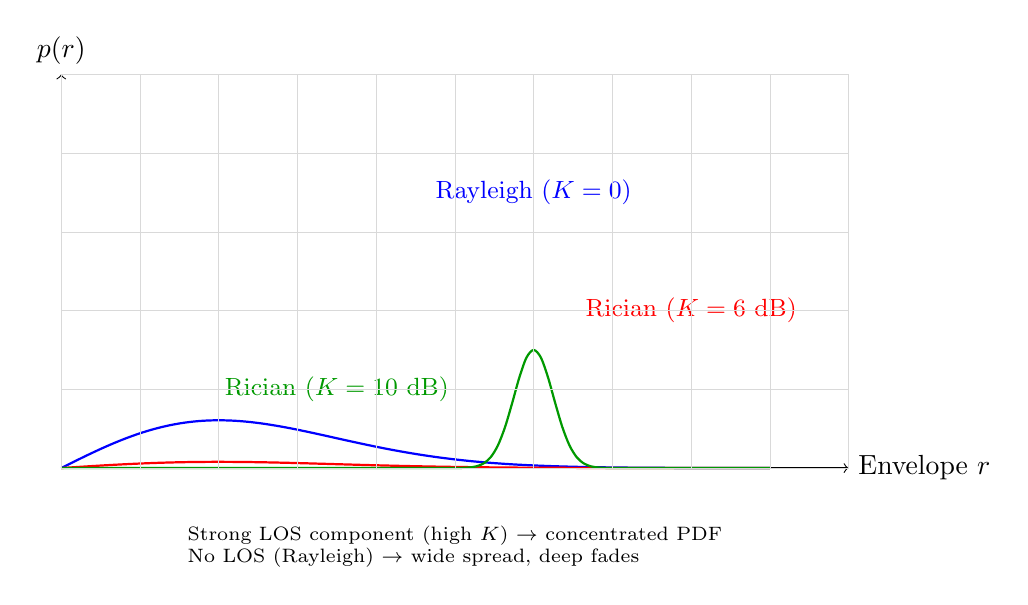
\begin{tikzpicture}[scale=1.0]
% Axes
\draw[->] (0,0) -- (10,0) node[right] {Envelope $r$};
\draw[->] (0,0) -- (0,5) node[above] {$p(r)$};

% Rayleigh PDF (K=0)
\draw[thick, blue, domain=0:9, samples=100, smooth] plot (\x, {(\x/2)*exp(-(\x*\x)/8)});
\node[blue, font=\small] at (6,3.5) {Rayleigh ($K=0$)};

% Rician K=6 dB (K=4)
\draw[thick, red, domain=0:9, samples=100, smooth] plot (\x, {0.8*(\x/2)*exp(-(\x*\x + 16)/8)*1.2});
\node[red, font=\small] at (8,2) {Rician ($K=6$~dB)};

% Rician K=10 dB (K=10) - more concentrated
\draw[thick, green!60!black, domain=0:9, samples=100, smooth] plot (\x, {(\x > 5 && \x < 7) ? 1.5*exp(-8*(\x-6)*(\x-6)) : 0});
\node[green!60!black, font=\small] at (3.5,1) {Rician ($K=10$~dB)};

% Grid
\draw[gray!30, very thin] (0,0) grid[step=1] (10,5);

% Annotations
\node[font=\scriptsize, align=left] at (5,-1) {
Strong LOS component (high $K$) $\rightarrow$ concentrated PDF\\
No LOS (Rayleigh) $\rightarrow$ wide spread, deep fades
};
\end{tikzpicture}
\end{center}

\subsection{Impact on BER}

Rayleigh fading \textbf{severely degrades} bit error rate performance. For \textbf{coherent BPSK} in Rayleigh fading:
\begin{equation}
\text{BER}_{\text{Rayleigh}} = \frac{1}{2}\left(1 - \sqrt{\frac{\bar{\gamma}}{1 + \bar{\gamma}}}\right)
\end{equation}
where:
\begin{itemize}
\item $\bar{\gamma} = \frac{E_b}{N_0}$ = average SNR per bit
\end{itemize}

Compare this to AWGN performance:
\begin{equation}
\text{BER}_{\text{AWGN}} = Q\left(\sqrt{2\bar{\gamma}}\right)
\end{equation}

\textbf{Comparison at $\bar{\gamma} = 10$~dB:}
\begin{itemize}
\item \textbf{AWGN channel}: BER = $3.9 \times 10^{-6}$
\item \textbf{Rayleigh fading}: BER = $0.005$ (\textbf{1000× worse!})
\end{itemize}

\begin{calloutbox}{Physical Explanation}
Deep fades push the instantaneous SNR into the noise floor, causing \textbf{error bursts}. Even though fades are brief, they dominate the average BER. This is why diversity and coding are essential for fading channels.
\end{calloutbox}

\subsection{Typical Rayleigh Environments}

Rayleigh fading is characteristic of:
\begin{itemize}
\item \textbf{Dense urban areas}: No LOS, many reflections from buildings (urban canyons)
\item \textbf{Indoor environments}: Office buildings, corridors, shopping malls
\item \textbf{Suburban/rural NLOS}: Heavy vegetation, obstructions blocking direct path
\item \textbf{Mobile-to-mobile communications}: Both terminals moving, no stable LOS
\end{itemize}

\section{Rician Fading}

\textbf{Rician fading} occurs when there is a \textbf{dominant line-of-sight (LOS) path} plus additional scattered components. The Rician distribution generalizes the Rayleigh distribution by adding a deterministic LOS component.

\subsection{Mathematical Description}

The \textbf{Rician PDF} is:
\begin{equation}
p_{\text{Ric}}(r) = \frac{r}{\sigma^2} \exp\left(-\frac{r^2 + A^2}{2\sigma^2}\right) I_0\left(\frac{Ar}{\sigma^2}\right), \quad r \geq 0
\end{equation}
where:
\begin{itemize}
\item $r$ = envelope amplitude
\item $A$ = amplitude of LOS component
\item $\sigma^2$ = average power of scattered components (per quadrature)
\item $I_0(\cdot)$ = modified Bessel function of the first kind, order zero
\end{itemize}

The \textbf{Rician K-factor} characterizes the ratio of LOS to scattered power:
\begin{equation}
K = \frac{A^2}{2\sigma^2} = \frac{\text{LOS power}}{\text{Scattered power}}
\end{equation}

In decibels:
\begin{equation}
K_{\text{dB}} = 10\log_{10}(K)
\end{equation}

\begin{keyconcept}
When $K = 0$ (no LOS), the Rician distribution \textbf{reduces to Rayleigh}. As $K \to \infty$ (pure LOS), the channel approaches AWGN. The K-factor thus interpolates between Rayleigh and AWGN behavior.
\end{keyconcept}

\subsection{Interpretation of K-factor}

\begin{center}
\begin{tabular}{lll}
\toprule
\textbf{K (dB)} & \textbf{Environment} & \textbf{Fading Severity} \\
\midrule
$-\infty$ ($K=0$) & No LOS (pure Rayleigh) & \textbf{Severe} (deep fades) \\
0~dB ($K=1$) & Equal LOS/scatter & Moderate \\
6~dB ($K=4$) & Strong LOS & Mild \\
10~dB ($K=10$) & Dominant LOS & Negligible fading \\
$+\infty$ & Pure LOS (AWGN-like) & None \\
\bottomrule
\end{tabular}
\end{center}

\begin{calloutbox}{Special Case: Rayleigh as Subset of Rician}
When $K = 0$ (no LOS component), the Rician distribution reduces to the Rayleigh distribution. Thus, Rician fading \textbf{generalizes} Rayleigh fading.
\end{calloutbox}

\subsection{Performance Impact}

\textbf{Rician fading is less severe than Rayleigh due to the dominant LOS component.}

\textbf{BPSK in Rician fading} (approximate):
\begin{equation}
\text{BER} \approx Q\left(\sqrt{\frac{2K\bar{\gamma}}{K+1}}\right) \exp\left(-\frac{K\bar{\gamma}}{K+1}\right) \times \text{(correction terms)}
\label{eq:bpsk-rician-ber}
\end{equation}

\textbf{Comparison at 10~dB average SNR:}
\begin{center}
\begin{tabular}{@{}lr@{}}
\toprule
Channel & BER \\
\midrule
\textbf{AWGN} & $3.9 \times 10^{-6}$ (best) \\
\textbf{Rician $K=6$~dB} & $\approx 10^{-5}$ (better than Rayleigh) \\
\textbf{Rayleigh ($K=0$)} & $0.005$ (worst) \\
\bottomrule
\end{tabular}
\end{center}

\subsection{Typical Rician Environments}

\begin{itemize}
\item \textbf{Suburban with partial LOS}
\item \textbf{Elevated antennas:} Rooftop installations
\item \textbf{Satellite-to-handheld:} Weak LOS plus ground reflections
\item \textbf{Indoor near windows:} Outdoor LOS plus indoor scatter
\end{itemize}

\section{Fade Depth \& Duration}

\subsection{Fade Margin}

\textbf{Link budget must include fade margin} to maintain target availability:
\begin{equation}
P_r(\text{min}) = P_r(\text{average}) - M_{\text{fade}}
\label{eq:fade-margin}
\end{equation}
where:
\begin{itemize}
\item $P_r(\text{min})$ = minimum received power for acceptable BER (dBm)
\item $P_r(\text{average})$ = average received power (dBm)
\item $M_{\text{fade}}$ = fade margin (dB)
\end{itemize}

\begin{calloutbox}{Example: Fade Margin Requirements}
Target 99\% availability (1\% outage):

\textbf{Rayleigh fading:}
\begin{itemize}
\item 10\% of time: signal $< -10$~dB below average
\item Need \textbf{10~dB margin} for 90\% availability
\item Need \textbf{20~dB margin} for 99\% availability
\end{itemize}

\textbf{Rician $K=6$~dB:} Fades less severe
\begin{itemize}
\item $\sim$5~dB margin for 90\%
\item $\sim$10~dB margin for 99\%
\end{itemize}
\end{calloutbox}

\subsection{Level Crossing Rate (LCR)}

\textbf{How often signal crosses threshold} (in fades/sec):
\begin{equation}
N_R = \sqrt{2\pi} f_d \rho \exp(-\rho^2)
\label{eq:level-crossing-rate}
\end{equation}
where:
\begin{itemize}
\item $N_R$ = level crossing rate (crossings/sec)
\item $f_d$ = maximum Doppler frequency (Hz)
\item $\rho = R/R_{\text{rms}}$ = normalized threshold (dimensionless)
\end{itemize}

\begin{calloutbox}{Example: Fade Rate}
Mobile at 100~km/h, 2~GHz ($f_d = 185$~Hz), threshold = average power ($\rho = 1$):
\begin{equation*}
N_R = \sqrt{2\pi} \times 185 \times 1 \times \exp(-1) \approx 85~\text{fades/sec}
\end{equation*}
The signal crosses the average power level 85 times per second!
\end{calloutbox}

\subsection{Average Fade Duration}

\begin{equation}
\bar{t} = \frac{\exp(\rho^2) - 1}{\rho f_d \sqrt{2\pi}}
\label{eq:average-fade-duration}
\end{equation}
where:
\begin{itemize}
\item $\bar{t}$ = average fade duration (s)
\end{itemize}

\begin{calloutbox}{Example: Fade Duration}
Same scenario as above (threshold = average power):
\begin{equation*}
\bar{t} = \frac{e - 1}{1 \times 185 \times \sqrt{2\pi}} \approx 3.7~\text{ms}
\end{equation*}

\textbf{Implication:} Fast fading (85 fades/sec), short fades ($\sim$4~ms) $\rightarrow$ Interleaving is effective.
\end{calloutbox}

\section{Mitigation Techniques}

\subsection{1. Diversity}

\textbf{Combine multiple independent fading signals to reduce probability of simultaneous deep fades.}

\begin{center}
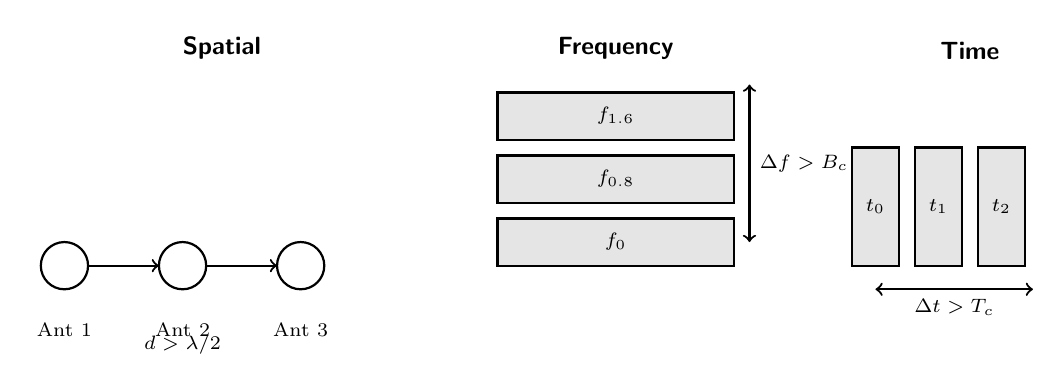
\begin{tikzpicture}[scale=1.0]
% Draw three diversity schemes
\begin{scope}[shift={(0,0)}]
\node[above,font=\sffamily\bfseries\small] at (2,2.5) {Spatial};
\draw[thick] (0,0) circle (0.3cm) node[below=0.6cm,font=\scriptsize] {Ant 1};
\draw[thick] (1.5,0) circle (0.3cm) node[below=0.6cm,font=\scriptsize] {Ant 2};
\draw[thick] (3,0) circle (0.3cm) node[below=0.6cm,font=\scriptsize] {Ant 3};
\draw[->,thick] (0.3,0) -- (1.2,0);
\draw[->,thick] (1.8,0) -- (2.7,0);
\node[font=\scriptsize] at (1.5,-1) {$d > \lambda/2$};
\end{scope}

\begin{scope}[shift={(5.5,0)}]
\node[above,font=\sffamily\bfseries\small] at (1.5,2.5) {Frequency};
\foreach \y in {0,0.8,1.6} {
  \draw[thick,fill=black!10] (0,\y) rectangle (3,\y+0.6);
  \node[font=\scriptsize] at (1.5,\y+0.3) {$f_{\y}$};
}
\draw[<->,thick] (3.2,0.3) -- (3.2,2.3) node[midway,right,font=\scriptsize] {$\Delta f > B_c$};
\end{scope}

\begin{scope}[shift={(10,0)}]
\node[above,font=\sffamily\bfseries\small] at (1.5,2.5) {Time};
\foreach \x in {0,1,2} {
  \draw[thick,fill=black!10] (\x*0.8,0) rectangle (\x*0.8+0.6,1.5);
  \node[font=\scriptsize] at (\x*0.8+0.3,0.75) {$t_{\x}$};
}
\draw[<->,thick] (0.3,-0.3) -- (2.3,-0.3) node[midway,below,font=\scriptsize] {$\Delta t > T_c$};
\end{scope}
\end{tikzpicture}
\end{center}

\subsubsection{Spatial Diversity (Antenna Diversity)}

\textbf{Separate antennas by $d > \lambda/2$:}

\textbf{Diversity gain:} $\sim$10~dB improvement with 2 antennas (selection combining).

\begin{calloutbox}{Example: WiFi Diversity}
WiFi access point with 2 antennas at 2.4~GHz ($\lambda = 12.5$~cm):
\begin{itemize}
\item Antenna spacing: 6~cm minimum
\item Result: Probability both antennas in deep fade is very low
\end{itemize}
\end{calloutbox}

\subsubsection{Frequency Diversity}

\textbf{Transmit same data on multiple frequencies} separated by $> B_c$.

\textbf{Application:} Frequency hopping spread spectrum (FHSS).

\subsubsection{Time Diversity}

\textbf{Transmit same data at different times} separated by $> T_c$.

\textbf{Implementation:} Interleaving + FEC (spread coded bits over time).

\subsection{2. Equalization}

\textbf{Compensate for frequency-selective fading (ISI).}

\subsubsection{Linear Equalization (LE)}

\textbf{Zero-forcing (ZF):} Invert channel response
\begin{equation}
H_{\text{eq}}(f) = \frac{1}{H_{\text{channel}}(f)}
\label{eq:zero-forcing}
\end{equation}
where:
\begin{itemize}
\item $H_{\text{eq}}(f)$ = equalizer frequency response
\item $H_{\text{channel}}(f)$ = channel frequency response
\end{itemize}

\textbf{Problem:} Noise amplification at deep fades.

\subsubsection{Decision-Feedback Equalization (DFE)}

\textbf{Use past decisions} to cancel ISI.

\textbf{Advantage:} Doesn't amplify noise as much as ZF.

\subsubsection{Adaptive Equalization}

\textbf{Track time-varying channel.}

\textbf{Algorithms:} LMS (Least Mean Squares), RLS (Recursive Least Squares).

\textbf{Training:} Periodic pilot symbols to update equalizer coefficients.

\subsection{3. OFDM}

\textbf{Divide wideband signal into many narrowband subcarriers.}

\textbf{Each subcarrier $< B_c$} $\rightarrow$ Flat fading per subcarrier.

\textbf{Per-subcarrier equalization:} Simple single-tap equalizer.

\subsection{4. Spread Spectrum}

\textbf{Spread signal over wide bandwidth.}

\textbf{Frequency diversity:} Different frequency components fade independently.

\subsection{5. Error Correction Coding}

\textbf{FEC protects against error bursts.}

\textbf{Interleaving:} Spread coded bits across time/frequency.

\begin{calloutbox}{Example: Interleaving Effectiveness}
Convolutional code + interleaver:
\begin{itemize}
\item Error burst of 10 bits $\rightarrow$ Spread across 100+ bit positions
\item Decoder sees isolated errors (easier to correct)
\end{itemize}
\end{calloutbox}

\section{Worked Examples}

\subsection{Example 1: Urban Cellular (900~MHz)}

\textbf{Problem:} Characterize the fading in a dense urban cellular environment.

\textbf{Given:}
\begin{itemize}
\item Environment: Dense urban, NLOS
\item Delay spread: $\tau_{\text{rms}} = 3~\mu$s
\item Mobile velocity: 30~km/h (8.33~m/s)
\item Carrier frequency: 900~MHz ($\lambda = 0.333$~m)
\item Fading type: Rayleigh
\end{itemize}

\textbf{Solution:}

\textbf{Step 1: Calculate coherence bandwidth}
\begin{equation*}
B_c = \frac{1}{5\tau_{\text{rms}}} = \frac{1}{5 \times 3 \times 10^{-6}} = 67~\text{kHz}
\end{equation*}

\textbf{Implication:} GSM channel (200~kHz) experiences frequency-selective fading $\rightarrow$ Equalizer needed.

\textbf{Step 2: Calculate Doppler frequency}
\begin{equation*}
f_d = \frac{v}{\lambda} = \frac{8.33}{0.333} = 25~\text{Hz}
\end{equation*}

\textbf{Step 3: Calculate coherence time}
\begin{equation*}
T_c = \frac{0.423}{2f_d} = \frac{0.423}{50} = 8.46~\text{ms}
\end{equation*}

\textbf{Implication:} Channel constant over $\sim$15 GSM symbols (0.577~ms/symbol) $\rightarrow$ Slow fading.

\subsection{Example 2: Suburban LTE (2.6~GHz)}

\textbf{Problem:} Analyze LTE performance in a suburban environment with partial LOS.

\textbf{Given:}
\begin{itemize}
\item Environment: Suburban, partial LOS
\item Delay spread: $\tau_{\text{rms}} = 0.5~\mu$s
\item Mobile velocity: 100~km/h (27.8~m/s)
\item Carrier frequency: 2.6~GHz ($\lambda = 0.115$~m)
\item Fading type: Rician $K=5$~dB
\item LTE resource block (RB) bandwidth: 180~kHz
\end{itemize}

\textbf{Solution:}

\textbf{Step 1: Calculate coherence bandwidth}
\begin{equation*}
B_c = \frac{1}{5\tau_{\text{rms}}} = \frac{1}{5 \times 0.5 \times 10^{-6}} = 400~\text{kHz}
\end{equation*}

\textbf{Implication:} LTE RB (180~kHz) $< B_c$ $\rightarrow$ Mostly flat fading per RB.

\textbf{Step 2: Calculate Doppler frequency}
\begin{equation*}
f_d = \frac{v}{\lambda} = \frac{27.8}{0.115} = 242~\text{Hz}
\end{equation*}

\textbf{Step 3: Calculate coherence time}
\begin{equation*}
T_c = \frac{0.423}{2f_d} = \frac{0.423}{484} = 0.87~\text{ms}
\end{equation*}

\textbf{Implication:} Channel changes over $\sim$12 OFDM symbols (71~$\mu$s/symbol) $\rightarrow$ Moderate fading, pilot-aided tracking required.

\section{Applications}

\subsection{Cellular Networks}
\begin{itemize}
\item \textbf{4G/5G:} OFDM with MIMO to combat multipath
\item \textbf{Handoff:} Manage transitions between cells as fading changes
\item \textbf{Power control:} Compensate for fast fading
\end{itemize}

\subsection{WiFi (IEEE 802.11)}
\begin{itemize}
\item \textbf{Indoor environments:} Severe multipath from walls and furniture
\item \textbf{MIMO:} Multiple antennas provide spatial diversity
\item \textbf{Channel sounding:} Periodic estimation of channel state
\end{itemize}

\subsection{Satellite Communications}
\begin{itemize}
\item \textbf{Land mobile satellite:} Rician fading with shadowing
\item \textbf{Diversity combining:} Overcome deep fades
\item \textbf{Interleaving:} Spread errors across time
\end{itemize}

\subsection{IoT and Sensor Networks}
\begin{itemize}
\item \textbf{Low-power operation:} Fade margin critical for reliability
\item \textbf{LoRaWAN:} Spread spectrum provides frequency diversity
\item \textbf{Zigbee:} DSSS with diversity for robustness
\end{itemize}

\section{Summary}

\begin{center}
\begin{tabular}{@{}llll@{}}
\toprule
\textbf{Parameter} & \textbf{Rayleigh} & \textbf{Rician ($K=6$~dB)} & \textbf{AWGN} \\
\midrule
LOS component & None & Dominant & Pure LOS \\
Fade depth (10\% time) & $-10$~dB & $-5$~dB & 0~dB \\
BER penalty @ 10~dB SNR & $1000\times$ & $10\times$ & $1\times$ (baseline) \\
Mitigation & Diversity, FEC & Moderate FEC & Minimal FEC \\
Typical environment & Dense urban, indoor & Suburban, elevated & Free space \\
\bottomrule
\end{tabular}
\end{center}

\begin{keyconcept}
\textbf{Multipath fading is the dominant impairment} in mobile/urban wireless communications. Rayleigh fading (no LOS) is severe, causing up to 1000$\times$ degradation in BER. Rician fading (with LOS) is moderate. Effective mitigation requires diversity, equalization, OFDM, and robust FEC. Understanding coherence bandwidth ($B_c$) and coherence time ($T_c$) is critical for system design.
\end{keyconcept}

\section{Further Reading}

\begin{itemize}
\item \textbf{Chapter:} Propagation Modes (Ground Wave, Sky Wave, Line-of-Sight)---LOS vs NLOS propagation
\item \textbf{Chapter:} Atmospheric Effects (Ionospheric, Tropospheric)---clear-air effects
\item \textbf{Chapter:} Signal-to-Noise Ratio (SNR)---fading reduces instantaneous SNR
\item \textbf{Chapter:} Bit Error Rate (BER)---fading degrades BER significantly
\item \textbf{Chapter:} QPSK Modulation---requires fade mitigation
\item \textbf{Chapter:} OFDM \& Multicarrier Modulation---combats frequency-selective fading
\item \textbf{Chapter:} Spread Spectrum (DSSS/FHSS)---provides frequency diversity
\item \textbf{Chapter:} LDPC Codes---robust error correction for fading channels
\end{itemize}
